\documentclass{beamer}

\usetheme{CambridgeUS}
\usecolortheme{beaver}

\usepackage{amsmath}
\usepackage{dsfont}

\usepackage{t1enc}
\usepackage{float}
\usepackage{graphicx}
\usepackage{verbatim}
\usepackage{subfigure}

\setbeamertemplate{itemize items}[default]
\setbeamertemplate{enumerate items}[default]

%\usepackage{beamerthemesplit}

%\setbeamerfont{structure}{family=\rmfamily,shape=\itshape} 

% IEEE transaction type bibliography
% Citations are numbered based on the order of appearance
\bibliographystyle{ieeetr}
% In the bibliography slide, numbers will not 
% appear by default in beamer. This will make 
% numbered bibliography.
%\setbeamertemplate{bibliography item}[text]

% Use abc in footnote
\renewcommand{\thefootnote}{\fnsymbol{footnote}}


\title[Utilizing Motion Sensor Data for Some Image Processing Applications]
%\hspace{55pt}
%\insertframenumber/\inserttotalframenumber]
{Utilizing Motion Sensor Data for Some Image Processing Applications}
\author[Saragadam R V Vishwanath]%IIT Madras \hspace{25pt} EE11S063]
{Saragadam R V Vishwanath (EE10B035)\\
\vspace{3pt}
\small{under the guidance of Prof.\ A. N. Rajagopalan}
}
%\vspace{15pt}
\institute[IIT Madras]{
Department of Electrical Engineering\\
IIT Madras}
\date{May 15, 2014}


% Set pdf props
\usepackage{hyperref}
\hypersetup
{
    pdfauthor={Saragadam R V Vishwanath (EE10B035)},
    pdfsubject={B.Tech project viva},
    pdftitle={Utilizing Motion Sensor Data for Some Image Processing Applications},
    pdfkeywords={btech,thesis,report,image processing,motion sensors, inertial sensors}
}

\setbeamertemplate{title page}[default][colsep=-4bp,rounded=true]

\begin{document}

\begin{frame}
\titlepage
\end{frame}

% An outline of how we want to present our results. Remember that we have only
% 15 slides in total. Hence, Introduction, 3 per project and conclusion will 
% complete it. The 3 per project slides can be split as follows:
% -- Introduction and what is the algorithm.
% -- Experimental results.
% -- Conclusion and reflection.

% Motivation ------------------------------------------------------------------- 
\begin{frame}{Motivation}
\begin{itemize}
	\item Computational photography now moving to ubiquitous mobiles
	\item Increased computational power. Hence, increased avenues.
	\item Additional data in the form of motion sensors. Increased scope
	of research.
	\item Flexible programming on the mobile camera. Ability to implement
	algorithms on the fly instead of offline computing.
\end{itemize}
\end{frame}

% What do we have --------------------------------------------------------------
\begin{frame}{What do we have in hand}
\begin{itemize}
	\item A mobile that is easy to program.
	\begin{itemize}
		\item Access to three-axis accelerometer.
		\item Access to 5 mp camera with variable focus, exposure time and resolution.
		\item Access to TCP communication for sending data to computer.
	\end{itemize}
	\vspace{0.4cm}
	\item A desktop computer that is very fast.
	\begin{itemize}
		\item Python for writing all the applications.
		\item WiFi dongle to receive data wireless.
	\end{itemize}
\end{itemize}
% Insert pictures here.
\end{frame}

% What did we try --------------------------------------------------------------
\begin{frame}{What did we try}
\begin{itemize}
	\item Image deblurring using semi-blind methods.
	\item Estimating depth using motion blur and shape from focus.
	\item Image registration for pure translation and pure rotation cases.
	\item A little of the image super-resolution.
\end{itemize}
\end{frame}

% Image deblurring -------------------------------------------------------------
\begin{frame}{Image Deblurring -- Primer}
\begin{itemize}
	\item Blur induced due to shake of the hand held camera. 
	\item Ill-posed if no more information is available.
	\item Idea is to get either the PSF directly or get a good initial
	estimate.
	\item Trajectory can be estimated using data from accelerometer. 
	\begin{itemize}
	\item No scene depth information. Hence we iterate through a possible set of 
	depths. 
	\item Drift due to erroneous gravity estimation. Hence we compensate by
	iterating through a set of possible drifts.
	\end{itemize}
\end{itemize}
\end{frame}

\begin{frame}{Image Deblurring -- Results}

Results of non-blind deconvolution using wiener deconvolution
\begin{figure}
\begin{center}
	\begin{subfigure}{Blurred image.}
		\resizebox{20mm}{!} {
\includegraphics {../images/deblur/imblur.png}}
	\end{subfigure}
	\begin{subfigure}{Image deblurred using wiener deconvolution.}
		\resizebox{20mm}{!} {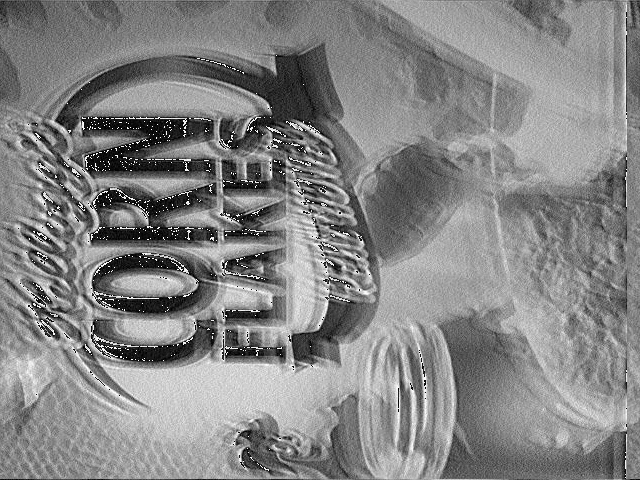
\includegraphics {../images/deblur/imdeblur.png}}
	\end{subfigure}
	\begin{subfigure}{Image deblurred using state of the art deconvolution algorithm.}
		\resizebox{20mm}{!} {
\includegraphics {../images/deblur/jia_blind_deconv.png}}
	\end{subfigure}
\end{center}
\end{figure}

Results of semi-blind deconvolution using Punnappurath et al's code.

\begin{figure}[H]
\begin{center}
\resizebox{20mm}{!} {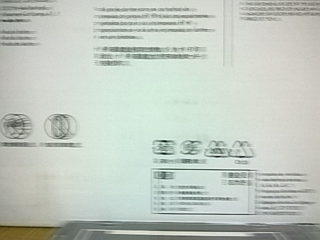
\includegraphics {../images/semiblind/blurred.png}}
\resizebox{20mm}{!} {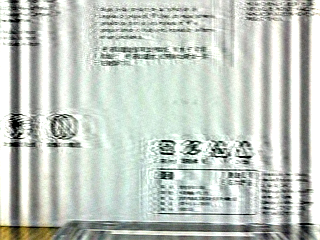
\includegraphics {../images/semiblind/blind.png}}
\resizebox{20mm}{!} {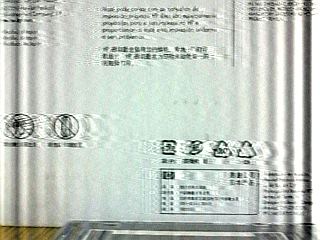
\includegraphics {../images/semiblind/semi_blind.png}}
\caption{Blurred image, image deconvolved by total blind method and image 
deconvolved by using our kernel as initial estimate.}
\end{center}
\end{figure}

\end{frame}
% End
\end{document}
